\textbf{I -- SVILUPPO DEI PEZZI E PERDITA DI TEMPI}

Molti di voi sapranno già che la partita suole dividersi in tre fasi ben
distinte: apertura, mediogioco e finale.

L'apertura è caratterizzata dallo ``sviluppo'' dei pezzi. Tengo qui a
sottolineare un primo concetto non spiegato a sufficienza in molti
manuali. Per \emph{sviluppo} non si intende il semplice spostamento dei
pezzi dalle loro case iniziali, piuttosto conferire ad essi \emph{una
funzione}. È ovvio che di norma per conferire ad un pezzo una funzione
occorre muoverlo, ma non di necessità.

Ogni manuale illustra invece a dovere l'importanza del centro: per
rendersi conto di quanto sia importante occupare con i pezzi le case
centrali basta riflettere che, per esempio, un Cavallo posto in una
delle quattro case centrali può andare in una casa d'angolo in due o tre
mosse mentre un Cavallo posto in una casa d'angolo impiega per andare in
un'altra casa d'angolo cinque o sei mosse. Chi ha i pezzi raggruppati
nella zona centrale può spostare in meno che non si dica forze ingenti
in ogni parte della scacchiera.

È ovvio che non è facile occupare il centro con i pezzi; i pezzi sono
facilmente scacciabili dai pedoni e finché ci sono pedoni arretrati
questa operazione è impossibile.

Nella fase iniziale della partita si assiste allora ad una lotta per lo
spazio centrale. Di solito i giocatori spingono al centro i pedoni in
modo da sviluppare indisturbati i propri pezzi nelle retrovie oppure
lasciano all'avversario la possibilità di occuparlo con i pedoni per poi
minarlo con spinte oculate.

Tipiche difese che contemplano questa strategia sono la Alekhine e la
Grünfeld.

Vediamo le prime mosse di entrambe:
\newgame
\emph{Alekhine:} \mainline{1.e4 Nf6 2.e5 Nd5 3.c4} (una variante meno
pretenziosa è 3.d4) \textbf{3... ¤b6 4.d4 d6 5.f4}

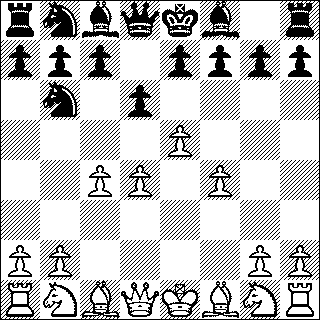
\includegraphics[width=1.50417in,height=1.50417in]{assets/diagrams/image1.png}\emph{diagramma
1}

\emph{Grünfeld:} \textbf{1.d4 ¤f6 2.c4 g6 3.¤c3 d5 4.¤xd5 ¤xd5 5.e4 ¤xc3
6.bxc3}

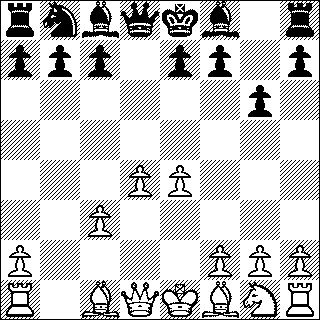
\includegraphics[width=1.50417in,height=1.50417in]{assets/diagrams/image2.png}\emph{diagramma
2}

In queste difese il Bianco è teso a comprimere l'avversario e a
sfruttare il vantaggio di spazio; il Nero lavora ai fianchi per minare
la struttura di pedoni nemica. Se ci riesce il crollo del centro ha di
solito effetti dirompenti perché potrà essere occupato da pezzi che non
potranno essere in alcun modo scacciati. \emph{"Ogni spinta di pedone
crea una debolezza"} ammoniva Steinitz.

Un altro elemento da tener presente è la velocità di mobilitazione delle
forze. Negli scacchi non si esce con un pezzo per fare azioni
dimostrative, saggiare la reazione del nemico e agire di conseguenza,
non se ne avrebbe il tempo! Si mobilitano invece le forze prima
possibile. Per fare questo si deve evitare di muovere senza necessità lo
stesso pezzo in apertura (andare in due mosse in una casa in cui si può
andare in una si dice ``perdere un tempo'').

Per sapere nelle prime mosse d'apertura chi è in vantaggio di sviluppo
c'è un metodo molto semplice: fare la conta dei pezzi sviluppati. Si sa
che il Bianco, avendo la prima mossa, è in vantaggio. In linea generale
dovrebbe riuscire a terminare la mobilitazione delle forze prima del
Nero.

Ammettiamo che le prime mosse di una partita siano \emph{1.e3 e5 2.e4} e
si noti che la stessa posizione si ottiene dopo \emph{1.e4 e5} ma con la
mossa al Bianco. Nel caso in esame è invece il Nero che può completare
lo sviluppo per primo e dopo \emph{2... ¤f6} egli ha già un pezzo
sviluppato contro nessuno del Bianco. In altre parole è bastato un solo
tempo perso per far passare il vantaggio (lieve quanto si vuole ma
innegabile) dal Bianco al Nero.

Per capire meglio questo concetto vediamo due esempi tratti dalla teoria
delle aperture.

\textbf{1.e4 e5 2.¤f3 ¤c6 3.¥b5} (Partita Spagnola)

\emph{diagramma 3}

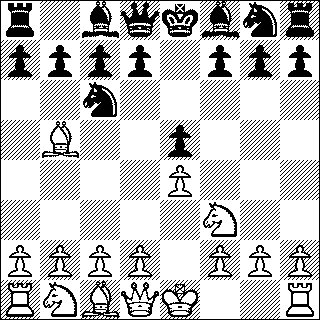
\includegraphics[width=1.50417in,height=1.50417in]{assets/diagrams/image3.png}

Questa è una buona mossa perché fa pressione sullo schieramento del Nero
sul lato di Donna. L'Alfiere in b5 è sì attaccabile dal pedone
avversario (per esempio con 3... a6) ma senza guadagno di tempo: dopo
\textbf{3... a6 4.¥a4} il Bianco ha ancora due pezzi sviluppati contro
uno solo del Nero.

Questo ci dà modo di chiarire il concetto: si ha guadagno di tempo solo
quando un pezzo è costretto a muoversi perché attaccato da un altro
pezzo o da un pedone centrale (mossa che, di solito, è utile all'uscita
dei pezzi.
Di per sé i pedoni si muovono non si sviluppano!).

Quando il Nero gioca 3... a6 il Nero fa più o meno questo ragionamento:
``Tu hai messo l'Alfiere in una posizione che comprime il mio lato di
Donna. Non mi piace per niente e intendo scacciarti, ma non subito, solo
quando lo decido io. Ora io gioco 3... a6 e ti costringo a scegliere tra
una delle seguenti possibilità:

a) a cambiare l'¥b5 con 4.¥xc6 ma allora rimango con il vantaggio dei
due Alfieri.

b) a spostarlo in a4 per continuare a esercitare la stessa pressione. In
tal caso però io sono pronto, quando lo riterrò opportuno, a scacciarti
con una semplice spinta di pedone (b7-b5).''

Dopo 3... a6 4. ¥a4 di solito a questo punto il Nero gioca \textbf{4...
¤f6}; non c'è infatti necessità di spingere subito in b5. Se il Bianco
avesse voluto prendere in c6 l'avrebbe fatto alla mossa precedente. Ora
sì che questa mossa sarebbe una perdita di tempo. Il Nero infatti,
rispetto a una mossa fa, ha mosso un Cavallo.

\emph{Difesa Scandinava:} \textbf{1.e4 d5 2.exd5 £xd5 3.¤c3!}

\emph{diagramma 4}

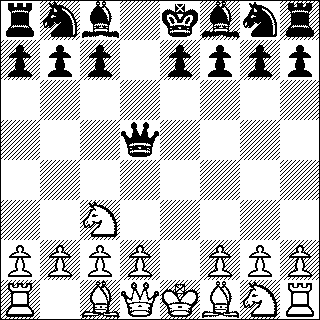
\includegraphics[width=1.50417in,height=1.50417in]{assets/diagrams/image4.png}

Questa mossa invece guadagna un tempo sul serio: costringe la Donna a
muoversi ancora e permette al Bianco di continuare lo sviluppo. Anche da
questo esempio traiamo un importante insegnamento: occorre attenzione
nel piazzare la Donna in apertura perché non potendo essere facilmente
barattata è costretta a muoversi ogni volta che incroci pezzi nemici.

La gravità della perdita di tempi non è costante ma dipende dal
carattere della posizione; se è chiusa, intendendo con questo termine
posizioni dove catene di pedoni dividono i due schieramenti, tale
perdita è meno grave. Nelle posizioni ``chiuse'' si assiste spesso a
manovre interne tese a portare i pezzi a contatto con i punti deboli
dell'avversario (gioco posizionale). Ne consegue che se un giocatore si
trova in vantaggio di sviluppo (caso tipico è quello di averlo già
completato mentre l'avversario ha ancora qualche mossa prima di poter
arroccare) allora deve aprire il gioco cambiando pedoni a tutta forza,
specie se centrali. Quanto più il vantaggio di sviluppo è marcato tanto
più è opportuno aprire le linee anche a costo di sacrificare materiale.
La forza d'urto della guerra lampo era già nota agli scacchisti prima
che Hitler nascesse!

Per finire vediamo una partita giustamente celebre in cui Paul Morphy,
mettendo in pratica questi semplici principi, acquisisce in poche mosse
un vantaggio decisivo e chiude con una combinazione brillante.

Morphy--Duca Karl e Conte Isouard, Parigi 1858.

\textbf{1.e4 e5 2.¤f3 d6} difende in e5. Questa mossa, che dà origine
alla Difesa Philidor è del tutto giocabile anche se non così buona come
la naturale 2... ¤c6 che pareggia il numero dei pezzi sviluppati.

\textbf{3. d4} il Bianco apre le linee per permettere uno sviluppo
arioso. Se ora il Nero prende in d4 (3... exd4) si priva del suo unico
baluardo centrale. In caso di presa ci si potrebbe chiedere come
riprendere il Pedone. Vale la pena soffermarci a riflettere che in
questa posizione esso potrà essere ripreso anche di Donna. Infatti la
casa d4 è meno esposta agli attacchi di quel che sembra. Scartato subito
l'attacco di pedone c7-c5 perché indebolisce in modo grave il Pd6 e crea
un ``buco'' in d5, il Bianco risponderebbe a 4... .¤c6 con 5. ¥b5! e se
5... .¥d7 6. ¥xc6 ¥xc6 7.¤c3 e i tre pezzi sviluppati (contro uno solo
del Nero) e l'occupazione delle case centrali ben compensano la rinuncia
alla coppia degli Alfieri. Non del tutto a torto molti preferiscono
anteporre, dopo 1.e4 e5 2.¤f3 d6 3.d4 exd4 4.£xd4, l'uscita d'Alfiere in
d7 alla mossa di Cavallo in c6.

\textbf{3... ¥g4} sembra una buona mossa ma non lo è. Il Nero difende il
Pe5 inchiodando il Cavallo e sviluppando un pezzo. In apparenza ha
ristabilito la parità nello sviluppo dei pezzi (uno per uno) ma \ldots{}

\textbf{4.£xe5 ¥xf3} forzata. Il Nero è costretto a privarsi dell'unico
pezzo sviluppato. Si consideri che la posizione è ``ariosa'' e che in
tali circostanze la coppia degli Alfieri è un bene cui non si rinuncia
senza compensi di altro genere; e qui non si vede che cosa il Nero abbia
ottenuto in cambio.

\textbf{5.£xf3 £xe5 6.¥c4 ¤f6 7.£d3} il Bianco rimuove la Donna per
piazzarla in una casa dove sviluppa la sua massima efficacia. Non si può
parlare di perdita di tempo perché le minacce su f7 e b7 costringono il
Nero a difendersi senza poter muovere un pezzo leggero.

\textbf{7... £e7} per poter rispondere a 8.£xb7 con 8... £d4+, cambiare
le Donne e tirarla in lungo.

Esaminiamo la posizione: sia il Bianco che il Nero hanno mosso due pezzi
ma che differenza! Quelli bianchi sono piazzati in case ideali mentre la
Donna nera intralcia lo sviluppo sul lato di Re e il Nero dovrà
necessariamente rimuoverla, con pe¢dita di tempi.

\textbf{8.¤c3!} ecco una mossa che all'epoca solo Morphy poteva giocare.
Altri avrebbero preso in b7 e dopo 8... £d4+ 9.c3 ¥c5 avrebbero forse
anche vinto ma dopo un lungo finale. Morphy capisce che non è il momento
di andare a caccia di pedoni ma di incrementare il vantaggio di
sviluppo.

\textbf{8... c6} non avendo più lo scacco in b4 il Nero difende il Pb7
ma questa è ancora una mossa di pedone.

\textbf{9.¥g5} ormai il vantaggio di sviluppo è schiacciante. Quattro
pezzi già piazzati nelle case migliori, le torri pronte ad entrare in
gioco tramite la colonna d. Per contro il Nero ha solo due pezzi mossi e
uno di essi dovrà essere rimosso perché impedisce lo sviluppo.

\textbf{9... b5 10.¤xb5} in queste condizioni il sacrificio è così
spontaneo che non abbisogna nemmeno di un calcolo preciso: non può
essere sbagliato!

\textbf{10... ¤xb5 11.¥xb5+ ¤bd7 12.0-0-0} l'attacco si sviluppa da sé.

\textbf{12... ¦d8}

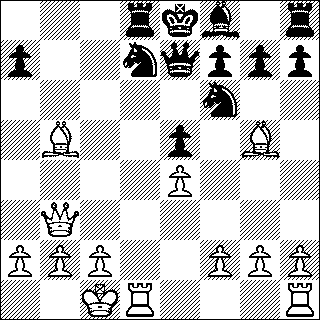
\includegraphics[width=1.50417in,height=1.50417in]{assets/diagrams/image5.png}

\emph{diagramma 5}

La partita è strategicamente vinta. Ora non rimane che il colpo tattico.

\textbf{13.¦xd7! ¦xd7 14.¦d1 £e6 s}e il nero invece di giocare 14...
.£e6 avesse mosso la Donna in d8 il Bianco avrebbe vinto con: 15.¥xd7+;
infatti:

\begin{enumerate}
\def\labelenumi{\alph{enumi})}
\item
  15. ... ¢e7 16.£a3 (o £d4) matto;
\item
  15. ... ¤xd7 16.¥xd8 ¢xd8 17.£d3 come se non bastasse, cade anche il
  Cavallo;
\item
  15. ... £xd7 16.¦xd7 anche non considerando che l'attacco non è ancora
  finito, il vantaggio di materiale del Bianco è più che sufficiente per
  vincere: due pedoni in più, un terzo (il \textbf{§}a7) indifendibile e
  la Donna vale di più di Alfiere e Torre.
\end{enumerate}

\textbf{15.¥xd7+ ¤xd7 16.£d8+!! ¤xb8 17.¦d8 matto.}

Come questa partita dimostra, la combinazione è la naturale conclusione
di una partita vinta innanzitutto dal punto di vista strategico.

A Morphy bastava applicare semplici concetti quali lo sviluppo e il
guadagno dei tempi, contro avversari che non li conoscevano ancora, per
terminare la partita con combinazioni spettacolari. La superiorità di
Morphy non risiedeva nella tattica, come si crede' a lungo, ma nella
strategia; la tattica non fu che un inevitabile corollario di questa
superiorità strategica.
